
\section{Sunset Combustion Code}



\begin{figure}[t]
\centering
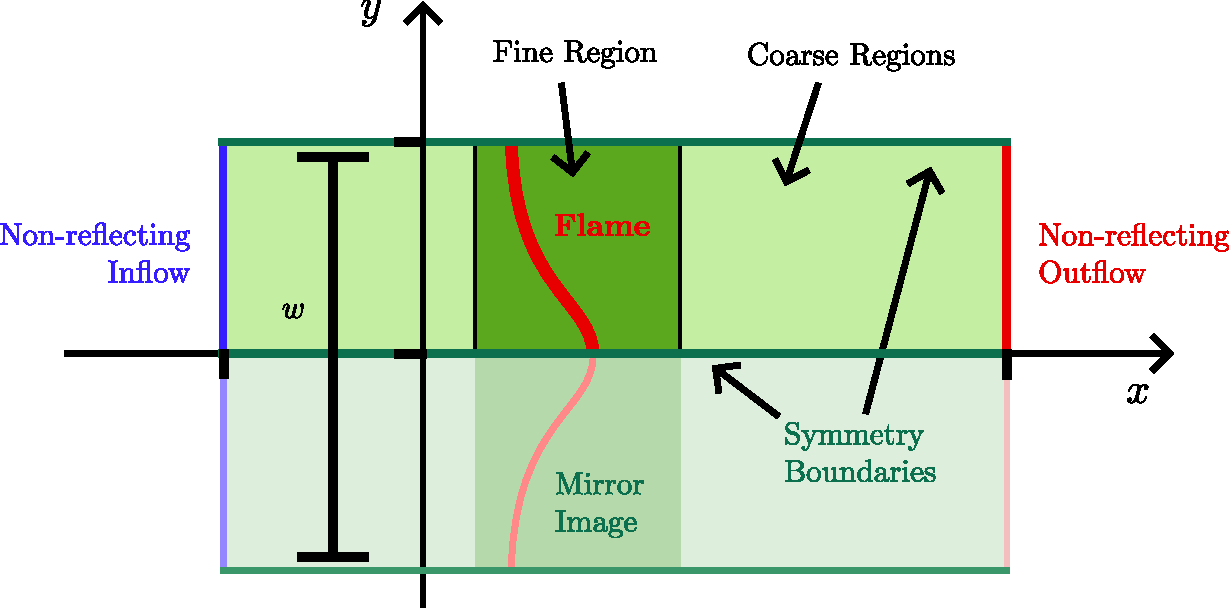
\includegraphics[scale=0.6]{assets/imgs/DNS-computational-domain.pdf}
\caption{DNS COMPUTATIONAL DOMAIN}
\label{fig:DNS-domain}
\end{figure}



\red{
we use the SUNSET code to perform combustion simulations [cite]

here are explanations of the methods used therein
}


\section{LABFM}

The \emph{Local Anisotropic Basis Function Method} (LABFM) \cite{king2024MeshFreeFrameworkHighOrder, king2020HighOrderDifference, king2024MeshfreeFrameworkHighorder, king2022HighorderSimulationsIsothermal, king2024SunsetFlamesDNSCode, broadley2025HighorderMeshfreeDirect, starepravo2025CanNeuralNetworks} is a high order spatial method used particularly in the computation of fluid flows. It allows for the calculation of arbitrary order approximations to spatial derivatives with arbitrary orders of accuracy, all on unstructured, mesh-free node sets. In keeping with the tradition set forth in prior methods (e.g. finite differences), polynomial interpolation is used as a first step before making derivative approximations. Specifically, we choose to set out the method in the context of making a high order interpolation based off finitely many discrete function values $\phi_j$, before extending this to high-order derivatives, where further assumptions can be made to simplify derivation


\subsection{High-Order Interpolations}

Consider a location $\vec{x}$ surrounded locally by finitely many nodes $\vec{x}_j \in \cl{S}(\vec{x})$ which are enumerated by $j \in \cl{N}(\vec{x})$, where $\abs{\vec{x} - \vec{x}_j} < h(\vec{x})$. Assume the function $\phi = \phi(\vec{x})$, which is only known at the points $\phi_j = \phi(\vec{x}_j)$, is \emph{smooth enough}.\footnote{Such that as many derivatives of $\phi$ as are used in the derivation below are available to us.} Then, we express the interpolated value $\phi(\vec{x})$ as a linear combination of the surrounding values $\phi_j$:
\begin{equation} \label{eqn:L}
L^{\rm{int}}[\phi](\vec{x}) \equiv \sum_{j \in \cl{N}(\vec{x})} \phi_j w^{\rm{int}}(\vec{x}, \vec{x}_j) \approx \phi(\vec{x}).
\end{equation}
To find the weights $w^{\rm{int}}(\vec{x}, \vec{x}_j)$, we will be evaluating $\phi_j$ by means of Taylor series via derivatives of $\phi$. Each derivative is a projection from the vector of derivatives of $\phi$:
\begin{equation}
\vv{D}[\phi] = \left(\phi, \pdv{\phi}{x}, \pdv{\phi}{x}, \pdv[2]{\phi}{x}, \pdv[2]{\phi}{x}{y}, \pdv[2]{\phi}{x}, \dots \right)^T
\quad \text{and} \quad
\vv{D}^k[\phi] = \left(\phi, \pdv{\phi}{x}, \pdv{\phi}{x}, \dots, \pdv[k]{\phi}{x}, \dots, \pdv[k]{\phi}{y} \right)^T,
\end{equation}
where we have assumed that $\phi$ is a scalar field over two spatial dimensions $\vec{x}=(x, y)$, although the method may be simply extended to any number of dimensions (with the caveat that the number of nodes required increases greatly with dimension). In this notation, interpolation becomes $\phi(\vec{x}) = \vv{D}[\phi](\vec{x}) \cdot \vv{C}^{\rm{int}} = \vv{D}^k[\phi](\vec{x}) \cdot \vv{C}^{\rm{int}, k}$ where $\vv{D}[\phi](\vec{x})$ is the vector $\vv{D}[\phi]$ evaluated at the location $\vec{x}$, $\vv{C}^{\rm{int}} = (1, 0, 0, 0, 0, 0, \dots)^T$ and $\vv{C}^{\rm{int}, k} = (1, 0, 0, \dots, 0)^T$, is of the same length as $\vv{D}^k$. Introducing the vectors of monomials:
\begin{equation}
\vv{X}(\vec{x}) = \left(1, x, y, \frac{1}{2!} x^2, xy, \frac{1}{2!} y^2, \dots \right)^T
\quad \text{and} \quad
\vv{X}^k(\vec{x}) = \left(1, x, y, \dots, \frac{1}{k!} x^k, \dots, \frac{1}{k!} y^k \right)^T.
\end{equation}
we can simplify down the Taylor expansion of $\phi$ around the point $\vec{x}$ for any $\vec{x}_j$ as:
\begin{subequations}
\begin{align}
\phi_j &= \phi(\vec{x}) + \pdv{\phi}{x}\bigg|_{\vec{x}} (x_j - x) + \pdv{\phi}{y} \bigg|_{\vec{x}} (y_j - y)  \\
& \qquad  \quad \ \, + \frac{1}{2!} \pdv[2]{\phi}{x}\bigg|_{\vec{x}} (x_j - x)^2 + \pdv[2]{\phi}{x}{y}\bigg|_{\vec{x}} (x_j - x) (y_j - y) + \frac{1}{2!} \pdv[2]{\phi}{y}\bigg|_{\vec{x}} (y_j - y)^2 + \dots \\
&= \vv{D}[\phi](\vec{x}) \cdot \vv{X} (\vec{x}_j - \vec{x}).
\end{align}
\end{subequations}
This may be truncated to $\phi_j \approx \vv{D}^k[\phi](\vec{x}) \cdot \vv{X}^k (\vec{x}_j - \vec{x})$ with $\cl{O}(h^{k + 1})$ truncation error. Hence, $k$ can be reinterpreted as the maximum order of polynomials $\phi(\vec{x})$ under this approximation which are exactly interpolated.

Rewriting \equ{eqn:L} in this formulation:
\begin{subequations}
\begin{align}
L^{\rm{int}}[\phi](\vec{x}) &= \vv{D}[\phi](\vec{x}) \, \cdot \sum_{j \in \cl{N}(\vec{x})} \vv{X} (\vec{x}_j - \vec{x}) w^{\rm{int}}(\vec{x}, \vec{x}_j) \\
&\approx \vv{D}^k[\phi](\vec{x}) \, \cdot \sum_{j \in \cl{N}(\vec{x})} \vv{X}^k (\vec{x}_j - \vec{x}) w^{\rm{int}}(\vec{x}, \vec{x}_j) \equiv \vv{D}^k[\phi](\vec{x}) \cdot \vv{B}^{\rm{int}, k}(\vec{x}) \\
&\approx \vv{D}^k[\phi](\vec{x}) \cdot \vv{C}^{\rm{int}, k}
\end{align}
\end{subequations}
So our problem now involves finding values of $w^{\rm{int}}(\vec{x}, \vec{x}_j)$ such that the \emph{vector of moments} $\vv{B}^{\rm{int}, k}(\vec{x})$ of $w^{\rm{int}}$ approximates $\vv{C}^{\rm{int}, k}$. For consistency, then, we require that the first component is independent of $h$:
\begin{equation}
1 = C^{\rm{int}, k}_0 \approx B^{\rm{int}, k}_0(\vec{x}) = \sum_{j \in \cl{N}(\vec{x})} w^{\rm{int}} (\vec{x}, \vec{x}_j),
\end{equation}
so $w^{\rm{int}} = \cl{O}(h^0)$, where the subscript zeroes represent the leading vector component. The resulting error in this approximation is the combined $\cl{O}(h^{k + 1})$ error of truncating the Taylor expansion of $\phi_j$ and approximating $w^{\rm{int}}$.

What's left is to find the weights of $w^{\rm{int}}$ for any point $\vec{x}$ and nodes $\vec{x}_j$. To do this, we separate $w^{\rm{int}}$ into some dependence of $\vec{x}$ on the anisotropic surrounding nodes from the action of interpolation, which will later be generalised to arbitrary derivatives. This is done by writing it as the weighted sum of some anisotropic basis functions:
\begin{equation}
w^{\rm{int}}(\vec{x}, \vec{x}_j) = \vv{W}^k(\vec{x}_j - \vec{x}) \cdot \vv{\Psi}^{\rm{int}, k}(\vec{x})
\end{equation}
where the anisotropy is seen in the dependence of $\vv{W}^k$ on $(\vec{x}_j - \vec{x})$ rather than $|\vec{x}_j - \vec{x}|$ (contrasting to the radial basis function, RBF, method). Assuming that $\vv{W}^k$ comprises some suitable \emph{anisotropic basis functions} (ABFs) \cite{king2022HighorderSimulationsIsothermal}, we must find the vector of weights $\vv{\Psi}^{\rm{int}, k}(\vec{x})$. This is done by substituting the new form into the vector of moments:
\begin{align}
\vv{C}^{\rm{int}, k}
\approx \vv{B}^{\rm{int}, k}(\vec{x})
= \left( \sum_{j \in \cl{N}(\vec{x})} \vv{X}^k (\vec{x}_j - \vec{x}) \otimes \vv{W}^k(\vec{x}_j - \vec{x}) \right) \cdot \vv{\Psi}^{\rm{int}, k}(\vec{x})
\equiv M(\vec{x}) \, \vv{\Psi}^{\rm{int}, k}(\vec{x})
\end{align}
where $M$ is a $n \times n$ matrix and $n$ is the number of components of $\vv{C}^{\rm{int}, k}$. The vector of weights $\vv{\Psi}^{\rm{int}, k}(\vec{x})$ is found when the linear system is solved. Carrying over the error terms from previous steps, we expect convergence on the order $(k + 1)$ as long as the matrix $M$ is well-posed and the values of nodes $\vec{x}_j$ are close enough to $\vec{x}$ such that $h$ is small.


\subsection{High-Order Derivatives}

\begin{figure}[t]
\centering
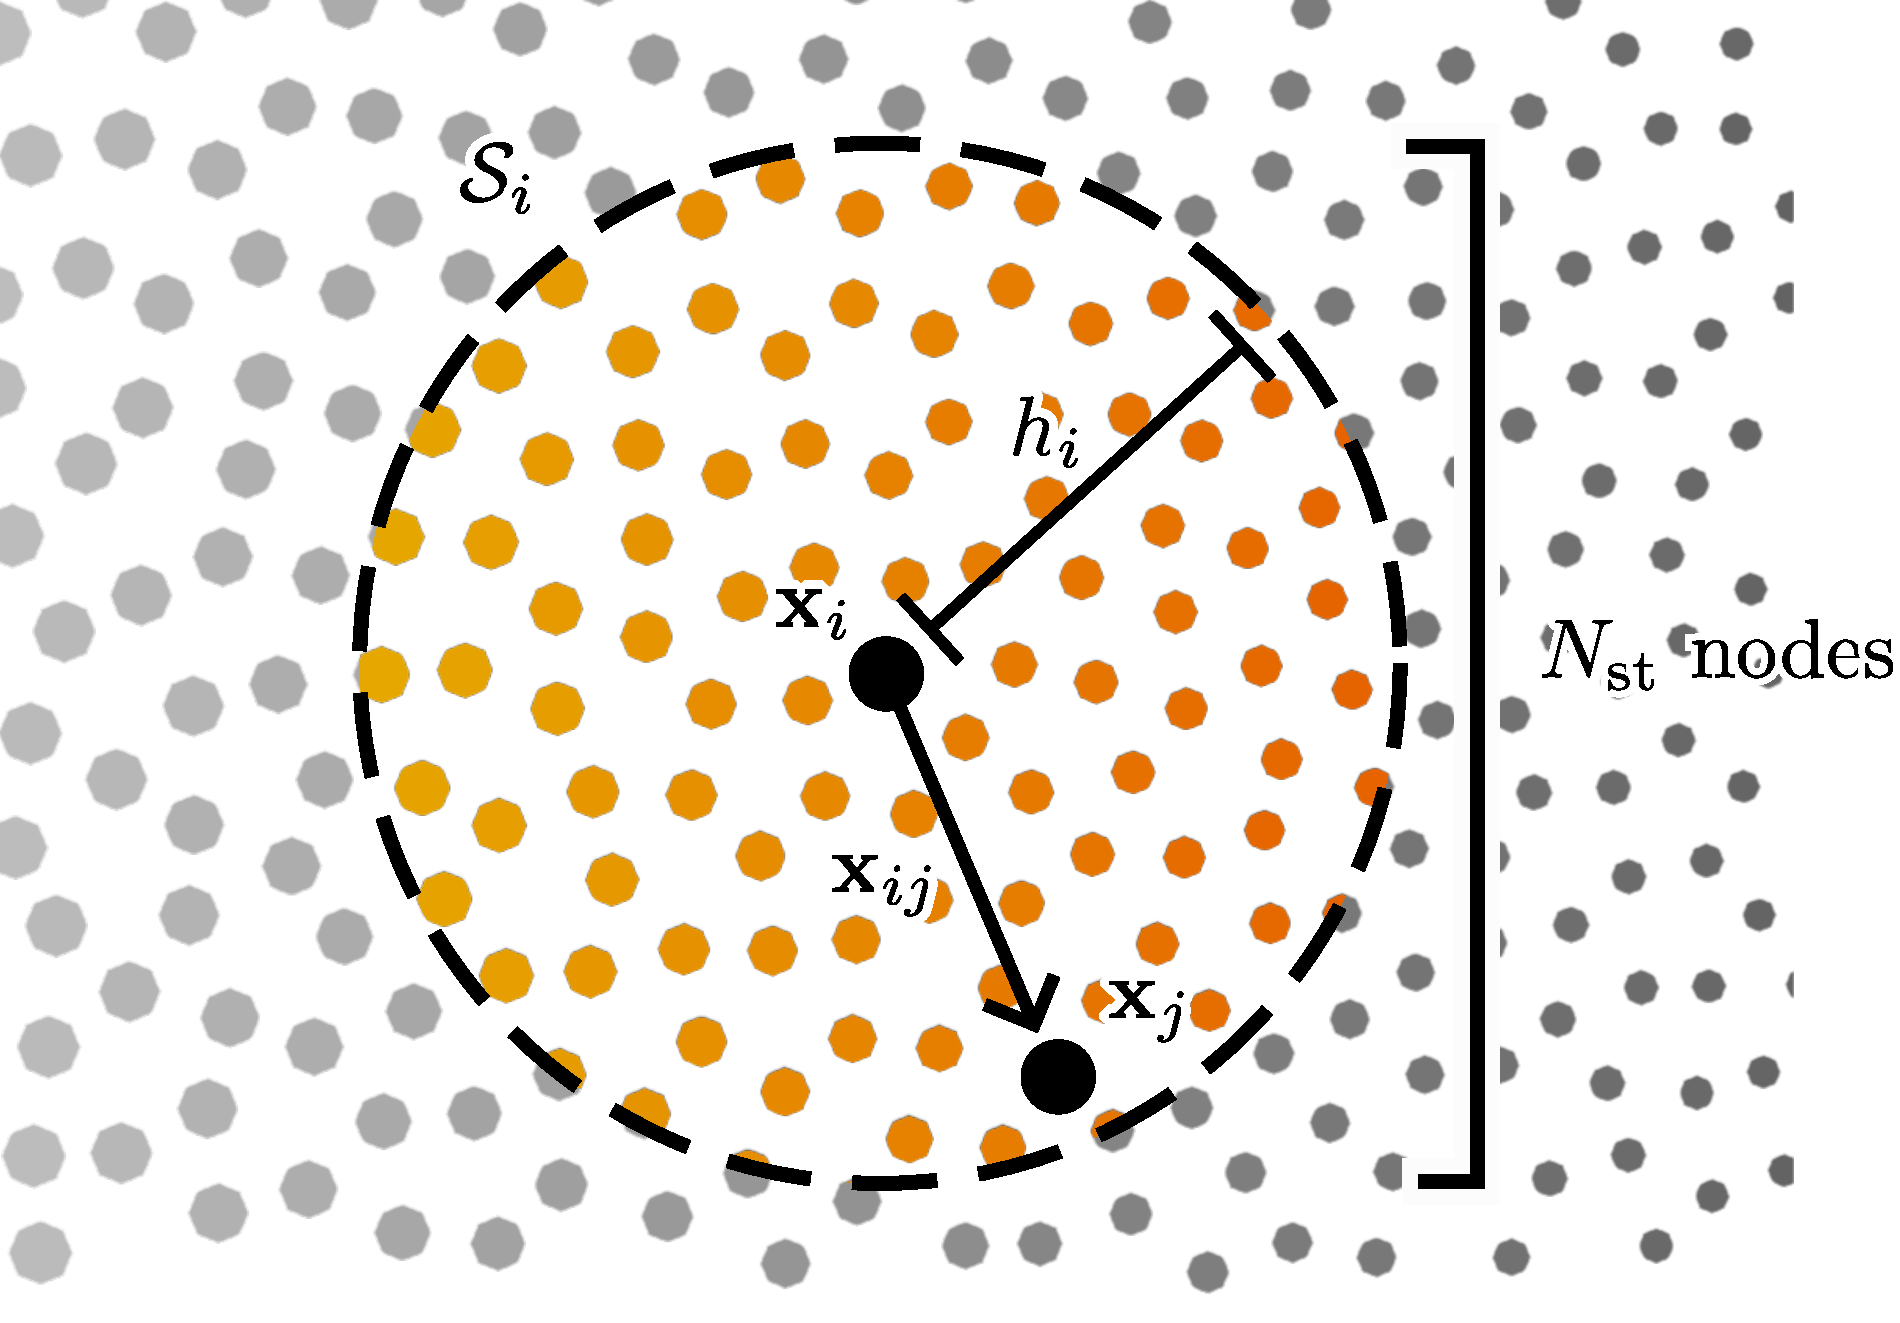
\includegraphics[scale=0.25]{assets/imgs/labfm-stencil-drawn_simple.pdf}
\caption{A example LABFM node discretisation and stencil.}
\label{fig:labfm-stencil}
\end{figure}

If we choose to evaluate a derivative at $\vec{x}$ instead, very little changes besides the following. Firstly, we assume that the point $\vec{x}$ is itself a node in our stencil, $\vec{x} = \vec{x}_i \in \cl{S}(\vec{x}_i)$, such that $\abs{\vec{x}_{ij}} < h_i$ for all $\vec{x}_j$ provided $\vec{x}_{ij} \equiv \vec{x}_j - \vec{x}_i$. An example discretisation and stencil is shown in \fig{fig:labfm-stencil}. Then, taking a page out of centred finite differences, we redefine our operator via the differences $\phi_{ij} \equiv \phi_j - \phi_i$:
\begin{equation} \label{eqn:labfm-L}
L[\phi]_i \equiv \sum_{j \in \cl{N}_i} \phi_{ij} w_{i, j}.
\end{equation}
This simplifies the derivation by removing the need to include leading order terms from our vectors. So now:
\begin{equation}
\vv{D}^k[\phi] \equiv \left(\pdv{\phi}{x}, \pdv{\phi}{x}, \dots, \pdv[k]{\phi}{x}, \dots, \pdv[k]{\phi}{y} \right)^T,
\qquad
\vv{X}^k_j \equiv \left(x_j, y_j, \dots, \frac{1}{k!} x_j^k, \dots, \frac{1}{k!} y_j^k \right)^T
\end{equation}
and similarly for $\vv{D}[\phi]$ and $\vv{X}_j$. For simplicity, we introduce the notation $\vv{X}^k_{ij} \equiv \vv{X}^k(\vec{x}_{ij})$. In this altered notation, the desired derivative is picked out through $\vv{C}^k$ and written as $\vv{D}^k[\phi] \cdot \vv{C}^k$. For example, a first derivative in $x$ has $\partial \phi / \partial x |_j = \vv{D}^k[\phi]_j \cdot \vv{C}^k$ where $\vv{C}^k = (1, 0, \dots, 0)^T$. Following the same logic as above, we find that
\begin{align}
L[\phi]_i
\approx \vv{D}^k[\phi]_i \, \cdot \sum_{j \in \cl{N}_i} \vv{X}^k_{ij} w_{i, j}
\equiv \vv{D}^k[\phi]_i \, \cdot \vv{B}^k_i \approx \vv{D}^k[\phi]_i \, \cdot \vv{C}^k
\end{align}
where we have reintroduced the vector of moments, $\vv{B}^k_i$, at node $\vec{x}_i$. As above, this approximation has $\cl{O}(h_i^{k + 1})$ truncation error. In this case, however, to ensure consistency we instead require $w_{i, j} = \cl{O}(h_i^d)$ where $d$ is the order of derivative we are approximating. This results in a $\cl{O}(h_i^{k + 1 - d})$ approximation thus far.

Once again, we represent the weights $w_{i, j}$ as a weighted average of the $k$ ABFs:
\begin{equation}
w_{i, j} = \vv{W}^k_{ij} \cdot \vv{\Psi}^k_i
\quad \text{where} \quad
\vv{W}^k_{ij} \equiv \vv{W}^k(\vec{x}_{ij})
\end{equation}
with the same form of linear system $\vv{C}^k = M_i \, \vv{\Psi}^k_i$ where $M_i \equiv \sum_{j \in \cl{N}_i} \vv{X}^k_{ij} \otimes \vv{W}^k_{ij}$. Once solutions to the linear system are found, we should have weights $w_{i, j}$ to order of accuracy $(k + 1 - d)$ provided again that $M_i$ is well-posed and $h_i$ remains small.




\subsection{Matrix Conditioning and Choice of ABFs}

The computational accuracy of the solutions in the linear system shown above is determined by the condition number of the matrix $M_i$. Given we expect any disordered set of nodes $\cl{S}_i$ close to $\vec{x}_i$ for the moment, there are no further assumptions we can make on $\vv{X}^k_{ij}$ yet. The choice of ABFs, however, can greatly improve the conditioning of $M_i$ by ensuring a linear independence of its columns, regardless of the order $k$ used. In particular, orthogonal basis functions do this automatically, such as the orthogonal Hermite and Legendre polynomials, and the Fourier basis modes -- combinations of $\sin(nx)$, $\cos(nx)$, $\sin(ny)$ and $\cos(ny)$ for different values of $n < k$.

It is also prudent to ensure that the weight values $w_{i ,j}$ do not change depending on the specific stencil size $h_i$ which we have taken. This is equivalent to ensuring the analysis may be done in a non-dimensional sense -- so derivative operators may be scaled to whatever dimensions are required in a particular simulation. In general, our ABFs already do not scale with $h_i$, but the vector of monomials $\vv{X}^k_{ij}$ does. We can cancel out this dependence by simply introducing the matrix $H_i = \rm{diag}(h, h, h^2, h^2, h^2, ..., h^k)$ and instead solving the system $H_i^{-1} \vv{C}^k = (H_i^{-1} M_i) \, \vv{\Psi}^k_i$ where instead $H_i^{-1} M_i = \sum_{j \in \cl{N}_i} (H_i^{-1} \vv{X}^k_{ij}) \otimes \vv{W}^k_{ij}$. This system condition number can no longer scale with $h_i$, since:
\begin{equation}
\left( H_i^{-1} \vv{X}^k_{ij} \right)_m
= h_i^{-n(m)} X^k_{ij, m}
\propto h_i^{-n(m)} \times h_i^{n(m)} = 1.
\end{equation}
The subscript $m$ is used for vector components, as above, and the index $n(m)$ is the order of monomial present at $X^k_{ij, m}$.



\subsection{Stencil Size, Computational Cost and Sampling}

One major advantage of LABFM and other unstructured methods, is that the distance between nodes, $\abs{\vec{x}_{ij}}$, and the resulting stencil size, $h_i$, is allowed to vary in space. This means we can move from a region of low-density nodes in, for example, a non-reacting part of our computational domain, to a high-density region where the flame is. But there is a limit to how fast this variation can occur, since any given order of polynomial reconstruction $k$, has $n(k)$ ABFs which must each be accurately sampled. Equivalently, this means we require at least one node per each of the $2k$ even slices of the circular stencil (each with angle $\pi / k$), assuming two-dimensions \cite{king2020HighOrderDifference}. This, of course, means that there is a practical lower limit to the number of nodes $N_{\rm{st}}$ required in a stencil which is well above the lower limit of $n(k)$ nodes required by compact methods like \cite{jensen1972FiniteDifferenceTechniques}. This results in a quadratic growth in required nodes as the slices get smaller, since $k \sim h_i \propto \sqrt{N_{\rm{st}}}$. Often, the stencil is increased furthermore to ensure a reliable sampling and improve stability and accuracy properties in spite of a strongly uneven node distribution. In a typical configuration, at $k = 4$ we may use $N_{\rm{st}} \approx 40$ and for $k = 6$ we may use $N_{\rm{st}} \approx 80$ \red{[CHANGE NUMBERS??]}. In three-dimensions this would be a cubic growth instead, since $k \sim h_i \propto \sqrt[3]{N_{\rm{st}}}$. Another obvious consequence of the sampling requirement, is that the order of LABFM used must be decreased at boundaries as no nodes are available to accurately sample the ABFs outside the computational domain.

Provided these conditions are met, this means we can approximate any derivative we like to arbitrary order simply by preprocessing the values of $w_{i, j}$ at each node\footnote{Only provided the nodes do not move. This precludes a Lagrangian formulation for LABFM.} and evaluating $L[\phi]_i$ during the simulation as we like. The preprocessing step is crucial as it means all that has to be done is calculate the sum in \equ{eqn:labfm-L} every time a derivative of an arbitrary function $\phi$ is required at a node $i$. The computational complexity of this operation is $\cl{O}(N_{\rm{st}})$. For a simulation of $N_{\rm{tot}}$ nodes, each with a constant stencil size of $N_{\rm{tot}}$ nodes, the cost becomes $\cl{O}(N_{\rm{tot}} N_{\rm{st}})$ to evaluate the same derivative of $\phi$ for each node.



\subsection{Operator Stability and Filtering}

Numerical approximations to differential operators such as the above contain error of two different behaviours: diffusive and dispersive. The former promotes the spurious damping of the signal, and the latter results in an incorrect phase velocity $c(\tilde{k})$ for a given wavenumber mode $\tilde{k}$ in the solution. These can be seen as the real and imaginary parts of eigenvalues to the linear stability problem concerning the operator. Unsurprisingly, the amplitude of these error terms gets smaller, faster, when the order of method increases. The same is true in the case of LABFM, with the unfortunate caveat that the higher order formulations result in eigenvalues which have positive real parts for the highest wavenumbers. This corresponds to an inverted diffusion effect for the shortest wavelength inaccuracies, such that any small floating-point errors destroy the simulation after only a few time steps. The natural solution to this, is to preprocess weights $w^{\rm{HV}}_{i, j}$ for a \emph{hyperviscosity} operator $-\D^2$, $\D^3$ or $-\D^4$ and apply this hyperviscosity at the end of each time step. This results in a filter where the wavenumber modes close to and above the \emph{Nyquist} wavenumber \cite{nyquist1928CertainTopicsTelegraph} are severely damped, without affecting the broader solution comprised of lower wavenumbers. Compared to other filtering methods, such as the direct removal of high wavenumber modes via spectral Fourier analysis, this has the obvious benefit of being easily calculated under the same LABFM formulation as the other derivatives (usually first- and second-order derivatives in the case of Navier-Stokes).






\section{Navier-Stokes Characteristic Boundary Conditions (NSCBC)}

% Include diffusive effects

% The first approximation made being for 


\subsection{The Locally One-Dimensional Inviscid (LODI) Approximation}

% Cite Thompson 1987, 1990, 1987 lectures?

Any hyperbolic system can be written in the form:
\begin{equation} \label{eqn:hyp-source}
\pdv{\und{U}}{t} + \vec{\nabla}\cdot\und{\vec{F}} + \und{B} = 0,
\end{equation}
where $\und{U}$ are the $N_\rm{V}$ conservative variables, $\und{\vec{F}}$ are the fluxes for each of these variables in each dimension and $\und{B}$ are source terms. Since we do not include diffusion effects, we assume that these terms are non-diffusive. % Also explain notation -> space in bold, variables underlined, matrices double underlined
This equation is unique up to linear combinations of the conserved variables, but can be transformed into a form for the primitive variables $\und{V}$, from which the characteristics will arise:
\begin{equation}
\pdv{\und{V}}{t} + \undt{\vec{A}} \cdot \vec{\nabla} \und{V} + \und{b} = 0
\end{equation}
where
\begin{equation}
P_{ij} \equiv \pdv{U_i}{u_j},
\quad
\boldsymbol{\Phi}_{ij} \equiv \pdv{\vec{F}_i}{u_j},
\quad
\undt{\vec{A}} \equiv \undt{P}^{-1}\undt{\boldsymbol{\Phi}}
\quad \text{and} \quad
\und{b} \equiv \undt{{P}}^{-1}\und{B}.
\end{equation}
The matrix $\undt{P}$ is the Jacobian matrix, $\undt{\vec{A}}$ represents the convection of the variables due to the other variables and themselves (e.g. resulting in $(\vec{u} \cdot \vec{\nabla})\vec{u}$ in the momentum equation) and $\und{\cl{S}}$ are source terms acting on primitive variables. Using this form, we can isolate the $x$-derivatives to observe the characteristics in that direction:
\begin{equation} \label{eqn:with_A}
\pdv{\und{V}}{t} + \undt{A}^x \pdv{\und{V}}{x} + \und{c} = 0
\quad \text{where, in 3D} \quad
\und{c} \equiv \und{b} + \undt{A}^y \pdv{\und{V}}{y} + \undt{A}^z \pdv{\und{V}}{z}
\quad \text{and} \quad
\und{C} \equiv \undt{P} \und{c}.
\end{equation}
The statement that the system is hyperbolic is now the statement that the $N_\rm{V}$ eigenvalues $\l_m = \l_m(\und{V})$ of $\undt{A}^x$ are real and can be ordered like $\l_1 \leq \dots \leq \l_{N_\rm{V}}$. Owing to this, we consider the left-eigenvectors $\und{l}_m = \und{l}_m(\und{V})$ of $\undt{A}^x$:
\begin{equation}
\und{l}_m^T \undt{A}^x = \l_m \und{l}_m^T.
\end{equation}
Multiplying equation \equ{eqn:with_A} by an eigenvector we project our equation into a solution space containing only the $m$\sus{th} characteristic invariant, $J_m$, which satisfies $\dd{J_m} = \und{l}_m^T \dd{\und{V}}$:
\begin{boxequ} \label{eqn:single_char_prob}
\und{l}_m^T \pdv{\und{V}}{t} + \l_m \und{l}_m^T \pdv{\und{V}}{x} + \und{l}_m^T \und{c} = 0,
\quad \iff \quad
\pdv{J_m}{t} + \l_m \pdv{J_m}{x} + \und{l}_m^T \und{c} = 0.
\end{boxequ}
We notice that along any trajectory $\vec{x}_m(t)$ which satisfies $\dd{\vec{x}_m}/\dd{t} = \l_m$ (i.e. the m\sus{th} characteristic has velocity $\l_m$), the invariant obeys:
\begin{equation}
\dv{J_m}{t} = - \und{l}_m^T \und{c}.
\end{equation}
This tells gives us an equation for each characteristic of the system, but numerically $J_m$ is not so useful since it needs to be transformed back into the primitive variables anyway for a simulation. Instead we use the form of the equation in primitive or conservative variables under the transformation $\undt{A}^x = \undt{S} \undt{\L} \undt{S}^{-1}$ where $\undt{\L}=\rm{diag}(\l_1, \dots, \l_{N_\rm{V}})$ is the diagonal matrix of eigenvalues and rows of the matrix $\undt{S}^{-1}$ are the corresponding \emph{left eigenvectors} $\und{l}_m^T$:
\begin{gather}
\cl{L}_m \equiv \l_m \pdv{J_m}{x} \equiv \l_m \und{l}_m^T \pdv{\und{V}}{x}, \\
\implies \quad
\boxed{
\pdv{\und{V}}{t} + \undt{S} \und{\cl{L}} + \und{c} = 0
\quad \text{and} \quad
\pdv{\und{U}}{t} + \undt{P} \undt{S} \und{\cl{L}} + \und{C} = 0,
}
\label{eqn:char-bcs-end}
\end{gather}
where $\und{\cl{L}} = (\cl{L}_1, \dots, \cl{L}_{N_\rm{V}})$. So each value $\cl{L}_m$ then represents the convection of the m\sus{th} characteristic wave at a point in space. The \emph{Locally One-Dimensional Inviscid} (LODI) characteristic boundary formulation\footnote{So-called as we preclude diffusive effects in any hyperbolic system of equations and we only observe characteristic waves moving over a boundary normal to a single dimension, i.e. not at a corner.} focuses on points at the boundary of a computational domain, and posits that outgoing characteristics through this boundary can be calculated as normal via upwinding, but characteristics entering the domain (such as an acoustic reflection) must instead be modelled. The key to LODI then, is that these incoming waves may be controlled by imposing their respective values of $\cl{L}_m$ at that boundary.

Note that, because we have the matrix $\undt{S}^{-1}$ not $\undt{S}$, we find the flux term $\und{d} \equiv \undt{S}\und{\cl{L}}$ by solving the linear system:
\begin{equation}
\undt{S}^{-1} \und{d} = \und{\cl{L}}.
\end{equation}




\subsection{Application to Reacting Flows}

Applying the LODI approximation to reacting equations first requires the form of their conservation equation. In three-dimensions, these are:
\begin{subequations}
\begin{alignat}{3}
\pdv{\r}{t} &+ \vec{\nabla} \cdot (\r \vec{u}) && &&= 0 \\
\pdv{\r \vec{u}}{t} &+ \vec{\nabla} \cdot (\r \vec{u}\otimes \vec{u} + p \bb{I}) && - \r \vec{g} &&= 0 \\
\pdv{\r e}{t} &+ \vec{\nabla} \cdot [(\r e + p) \vec{u}] && - \r \vec{g} \cdot \vec{u} &&= 0 \\
\pdv{\r Y_\a}{t} &+ \vec{\nabla} \cdot [\r Y_\a \vec{u}] && - \dot{\w}_\a &&= 0
\end{alignat}
\end{subequations}
for $\a = 1, \dots, N_{\rm{S}}$. The energy $e$ modelled here is the internal inergy rather than the total energy specified in \chap{ch:govern-eqns}. The algebraic equations for ideal gas and internal energy (so we ignore the constant chemical potential) for closure are:
\begin{equation}
\r e = \r E_{\rm{th}} + \r E_{\rm{ki}},
\quad \text{where} \quad
\r E_{\rm{th}} = \frac{p}{\gamma - 1}
\quad \text{and} \quad
\r E_{\rm{ki}} = \frac{1}{2} \r \vec{u} \cdot \vec{u}.
\end{equation}
In this case, the vectors of conservative variables, fluxes and source terms are:
\begin{equation}
\und{U} = \begin{pmatrix} \r \\ \r u^x \\ \r u^y \\ \r u^z \\ \r e  \\ \r Y_1 \\ \vdots \end{pmatrix},
\quad
\und{V} = \begin{pmatrix} \r \\ u^x \\ u^y \\ u^z \\ e \\ Y_1 \\ \vdots \end{pmatrix},
\quad
\und{F}^x = \begin{pmatrix} \r u^x \\ \r u^x u^x + p \\ \r u^x u^y \\ \r u^x u^z \\ (\r e + p) u^x \\ \r Y_1 u^x \\ \vdots \end{pmatrix},
\quad \text{and} \quad
\und{B} = \begin{pmatrix} 0 \\ - \r g^x \\ - \r g^y \\ - \r g^z \\ - \r \vec{g} \cdot \vec{u} \\ -\dot{\w}_1 \\ \vdots \end{pmatrix}.
\end{equation}
Hence, we evaluate the relevant matrices:
\begin{equation}
\undt{P} = \begin{pmatrix}
1   & 0  & 0 & 0 & 0 & 0 &  \\
u^x & \r & 0 & 0 & 0 & 0 &  \\
u^y & 0 & \r & 0 & 0 & 0 & \cdots \\
u^z & 0 & 0 & \r & 0 & 0 &  \\
\frac{1}{2} \vec{u} \cdot \vec{u} & \r u^x & \r u^y & \r u^z & 1/(\g - 1) & 0 & \\
Y_1 & 0 & 0 & 0 & 0 & \r & \\
 &  & \vdots &  &  &  & \ddots
\end{pmatrix}
\end{equation}
so
\begin{equation}
\undt{A}^x = \begin{pmatrix}
u^x & \r & 0 & 0 & 0 & 0 & \\
0 & u^x & 0 & 0 & 1 / \r & 0 & \\
0 & 0 & u^x & 0 & 0 & 0 & \\
0 & 0 & 0 & u^x & 0 & 0 & \\
0 & \g p & 0 & 0 & u^x & 0 &  \\
0 & 0 & 0 & 0 & 0 & u^x & \\
 &  & \vdots &  &  &  & \ddots
\end{pmatrix}
\quad \text{and} \quad
\und{b} = \begin{pmatrix} 0 \\ -g^x \\ -g^y \\ -g^z \\ 0 \\ -\dot{\w}_1 / \r \\ \vdots\end{pmatrix}.
\end{equation}
This gives us the full equations in the primitive variables, the full form of which is omitted. Considering the eigenvalue problem of $\undt{A}^x$, we have:
\begin{subequations}
\begin{alignat}{5}
\l_1 &= u^x - c  \qquad && \und{l}^T_1 &&= (0, -\r c, 0, 0, 1, 0, \dots) \quad && \text{and} \quad \cl{L}_1 &&= \l_1 \left(\pdv{p}{x} - \r c \pdv{u^x}{x}\right), \\
\l_2 &= u^x      \qquad && \und{l}^T_2 &&= (c^2, 0, 0, 0, -1, 0, \dots)  \quad && \text{and} \quad \cl{L}_2 &&= \l_2 \left(c^2 \pdv{\r}{x} - \pdv{p}{x}\right), \\
\l_3 &= u^x      \qquad && \und{l}^T_3 &&= (0, 0, 1, 0, 0, 0, \dots)     \quad && \text{and} \quad \cl{L}_3 &&= \l_3 \pdv{u^y}{x}, \\
\l_4 &= u^x      \qquad && \und{l}^T_4 &&= (0, 0, 0, 1, 0, 0, \dots)     \quad && \text{and} \quad \cl{L}_4 &&= \l_4 \pdv{u^z}{x}, \\
\l_5 &= u^x + c  \qquad && \und{l}^T_5 &&= (0, \r c, 0, 0, 1, 0, \dots)     \quad && \text{and} \quad \cl{L}_5 &&= \l_5 \left(\pdv{p}{x} + \r c \pdv{u^x}{x}\right), \\
\l_{5 + 1} &= u^x      \qquad && \und{l}^T_{5 + 1} &&= (0, 0, 0, 0, 0, 1, \dots)     \quad && \text{and} \quad \cl{L}_{5 + 1} &&= \l_{5 + 1} \pdv{Y_1}{x}
\end{alignat}
\end{subequations}
and so on. For the inverse problem:
\begin{subequations}
\begin{alignat}{5}
& \pdv{\r}{x}   &&= \frac{1}{c^2} \left[ \frac{\cl{L}_2}{\l_2} + \frac{1}{2} \left( \frac{\cl{L}_5}{\l_5} + \frac{\cl{L}_1}{\l_1} \right) \right] && \quad \text{and} \quad && d_1 &&= \frac{1}{c^2}\left[\cl{L}_2 + \frac{1}{2} \left( \cl{L}_5 + \cl{L}_1 \right) \right], \\
& \pdv{u^x}{x} &&= \frac{1}{2 \r c}\left(\frac{\cl{L}_5}{\l_5} - \frac{\cl{L}_1}{\l_1}\right) && \quad \text{and} \quad && d_2 &&= \frac{1}{2 \r c}(\cl{L}_5 - \cl{L}_1), \\
& \pdv{u^y}{x} &&= \frac{\cl{L}_3}{\l_3} && \quad \text{and} \quad && d_3 &&= \cl{L}_3, \\
& \pdv{u^z}{x} &&= \frac{\cl{L}_4}{\l_4} && \quad \text{and} \quad && d_4 &&= \cl{L}_4, \\
& \pdv{p}{x}   &&= \frac{1}{2}\left(\frac{\cl{L}_5}{\l_5} + \frac{\cl{L}_1}{\l_1}\right) && \quad \text{and} \quad && d_5 &&= \frac{1}{2}(\cl{L}_5 + \cl{L}_1), \\
& \pdv{Y_1}{x} &&= \frac{\cl{L}_{5 + 1}}{\l_{5 + 1}} && \quad \text{and} \quad && d_{5 + 1} &&= \cl{L}_{5 + 1}
\end{alignat}
\end{subequations}
and so on. Evidently, the eigenvalues $\l_1$ and $\l_5$ correspond to the speed of sound but since positive $x$ points into the domain, only one of these corresponds to an acoustic wave entering the domain.


\subsection{Non-Reflecting Subsonic Boundaries}

\subsubsection{Outflows}

The first non-reflective boundaries under this formulation come from \cite{thompson1987TimeDependentBoundary} in the case of the one-dimensional, subsonic, inviscid, non-isothermal Euler equations (the equations above if we lower the dimension of $\vec{x}$ and $\vec{u}$ and drop the mass fraction equations). This was promptly extended to the set of equations shown above in \cite{poinsot1992BoundaryConditionsDirect} for reacting flows. In both cases, a simple condition for acoustically non-reflecting boundaries was found by requiring that the Riemann invariant corresponding to the entering acoustic wave remain constant under the assumption that transverse terms can be neglected. At a subsonic outflow boundary on the left end of the computational domain, where $0 < u^x < c$, this means the invariant $J_5$ should remain constant at the boundary, provided transverse derivatives vanish. Equivalently, we require
\begin{equation}
0 = \und{l}^T_5 \pdv{\und{V}}{t} = \left( \pdv{p}{t} + \r c \pdv{u^x}{t} \right)
\end{equation}
given that, from equation \equ{eqn:single_char_prob}:
\begin{equation}
0 = \und{l}^T_5 \pdv{\und{V}}{t} + \cl{L}_5 + \und{l}^T_5 \und{b} = \left( \pdv{p}{t} + \r c \pdv{u^x}{t} \right) + \cl{L}_5 - \r c g^x.
\end{equation}
So we must enforce $\cl{L}_5 = \r c g^x$. Similarly, a subsonic outflow at the right end of the computational domain requires $\cl{L}_1 = - \r c g^x$.

\subsubsection{Inflows}

For subsonic outflows, regardless which side of the domain they reside, the only characteristic wave which enters the domain are either $\cl{L}_5$ for left-side boundaries and $\cl{L}_1$ for right-side boundaries. All the other $\cl{L}_m$ values required in \equ{eqn:char-bcs-end} may be found via the one-sided derivatives mentioned above



\subsection{Extra Boundary Considerations}

% What specifically is used in the code
% - Diffusive conditions (zero normal flux...) [Sutherland and Kennedy]
% - Yoo and Im tangential convection term
% - P controlled inflow/outflow
% - Wall boundaries






